\documentclass[tikz,border=8pt]{standalone}
% Shared look for every TikZ diagram. Load with \input{../../tools/tikz-style.tex}
\usepackage[T1]{fontenc}
\usepackage{lmodern}
\renewcommand{\sfdefault}{lmr}  % diagrams use the same serif as the text
\usetikzlibrary{arrows.meta, positioning, shapes.geometric, calc, fit, backgrounds}
\definecolor{cblue}{HTML}{4C78A8}
\definecolor{corange}{HTML}{F58518}
\definecolor{cgreen}{HTML}{54A24B}
\definecolor{cred}{HTML}{E45756}
\definecolor{cpurple}{HTML}{B279A2}
\definecolor{cgrey}{HTML}{6B6B6B}
\tikzset{
  every picture/.style={font=\sffamily, line width=1.2pt},
  box/.style={draw=#1, fill=#1!12, rounded corners=4pt, align=center, inner sep=7pt, minimum height=1.1cm},
  box/.default=cgrey,
  arrow/.style={-{Stealth[length=3mm]}, draw=cgrey, line width=1.4pt},
  title/.style={font=\sffamily\bfseries\Large},
  note/.style={font=\sffamily\small, text=cgrey, align=center},
}
\AtBeginDocument{\hyphenpenalty=10000 \exhyphenpenalty=10000}

\begin{document}
\begin{tikzpicture}[mat/.style={draw, thick, fill=#1, minimum width=0.55cm}]
  % X
  \node[mat=cblue!15, minimum height=3cm, minimum width=2.2cm] (X) {$X$};
  \node[note, below=0.1cm of X] {$m \times (n{+}1)$};
  \node[note, above=0.1cm of X, text width=3cm] {one row per point; first column all 1s};
  \node[right=0.15cm of X] (dot) {$\cdot$};
  \node[mat=corange!20, minimum height=2.2cm, right=0.15cm of dot] (w) {$w$};
  \node[note, below=0.1cm of w] {$(n{+}1) \times 1$};
  \node[right=0.2cm of w] (eq) {$=$};
  \node[mat=cblue!8, minimum height=3cm, right=0.2cm of eq] (z) {$z$};
  \node[note, below=0.1cm of z] {$m \times 1$};
  \draw[arrow] (z.east) -- node[above, note] {sigmoid} ++(1.6,0) node[right, mat=cgreen!20, minimum height=3cm] (yh) {$\hat{y}$};
  \node[note, below=0.1cm of yh] {$m \times 1$};
  % gradient
  \node[below=1.7cm of X, xshift=2.2cm, align=left] (g) {$\dfrac{\partial L}{\partial w} = -\dfrac{1}{m}\, X^{\mathsf T}(y - \hat{y})$};
  \node[note, right=0.4cm of g, text width=5.2cm, align=left] {$X^{\mathsf T}$ is $(n{+}1) \times m$, $(y - \hat{y})$ is $m \times 1$:\\ the gradient is $(n{+}1) \times 1$, one slope per weight, the same shape as $w$};
\end{tikzpicture}
\end{document}
